\subsubsection{05.02.2016}
\textit{\textbf{Time frame:}} 12:00-21:00 

This day we participated in a friendly match which took place in the Nizhny Novgorod. There was total of 3 teams in this meeting, so the matches were held 1 vs 1. Our team got the second place in this competition. 

\begin{figure}[H]
	\begin{minipage}[h]{0.47\linewidth}
		\center{\includegraphics[scale=0.17]{3Engineering/5Team_meetings/days_of_meetings/2016.02.05/images/01}}
		\caption{Match}
	\end{minipage}
	\hfill
	\begin{minipage}[h]{0.47\linewidth}
		\center{\includegraphics[scale=0.15]{3Engineering/5Team_meetings/days_of_meetings/2016.02.05/images/02}}
		\caption{Match}
	\end{minipage}
\end{figure}

During the competition there were found some problems in the robot. 

The first problem was that the protection around the bucket prevented the bucket from getting inside the robot. To avoid this, the protection was adjusted to the needed dimensions. Since then the bucket could get inside the robot without difficulties.

\begin{figure}[H]
	\begin{minipage}[h]{1\linewidth}
		\center{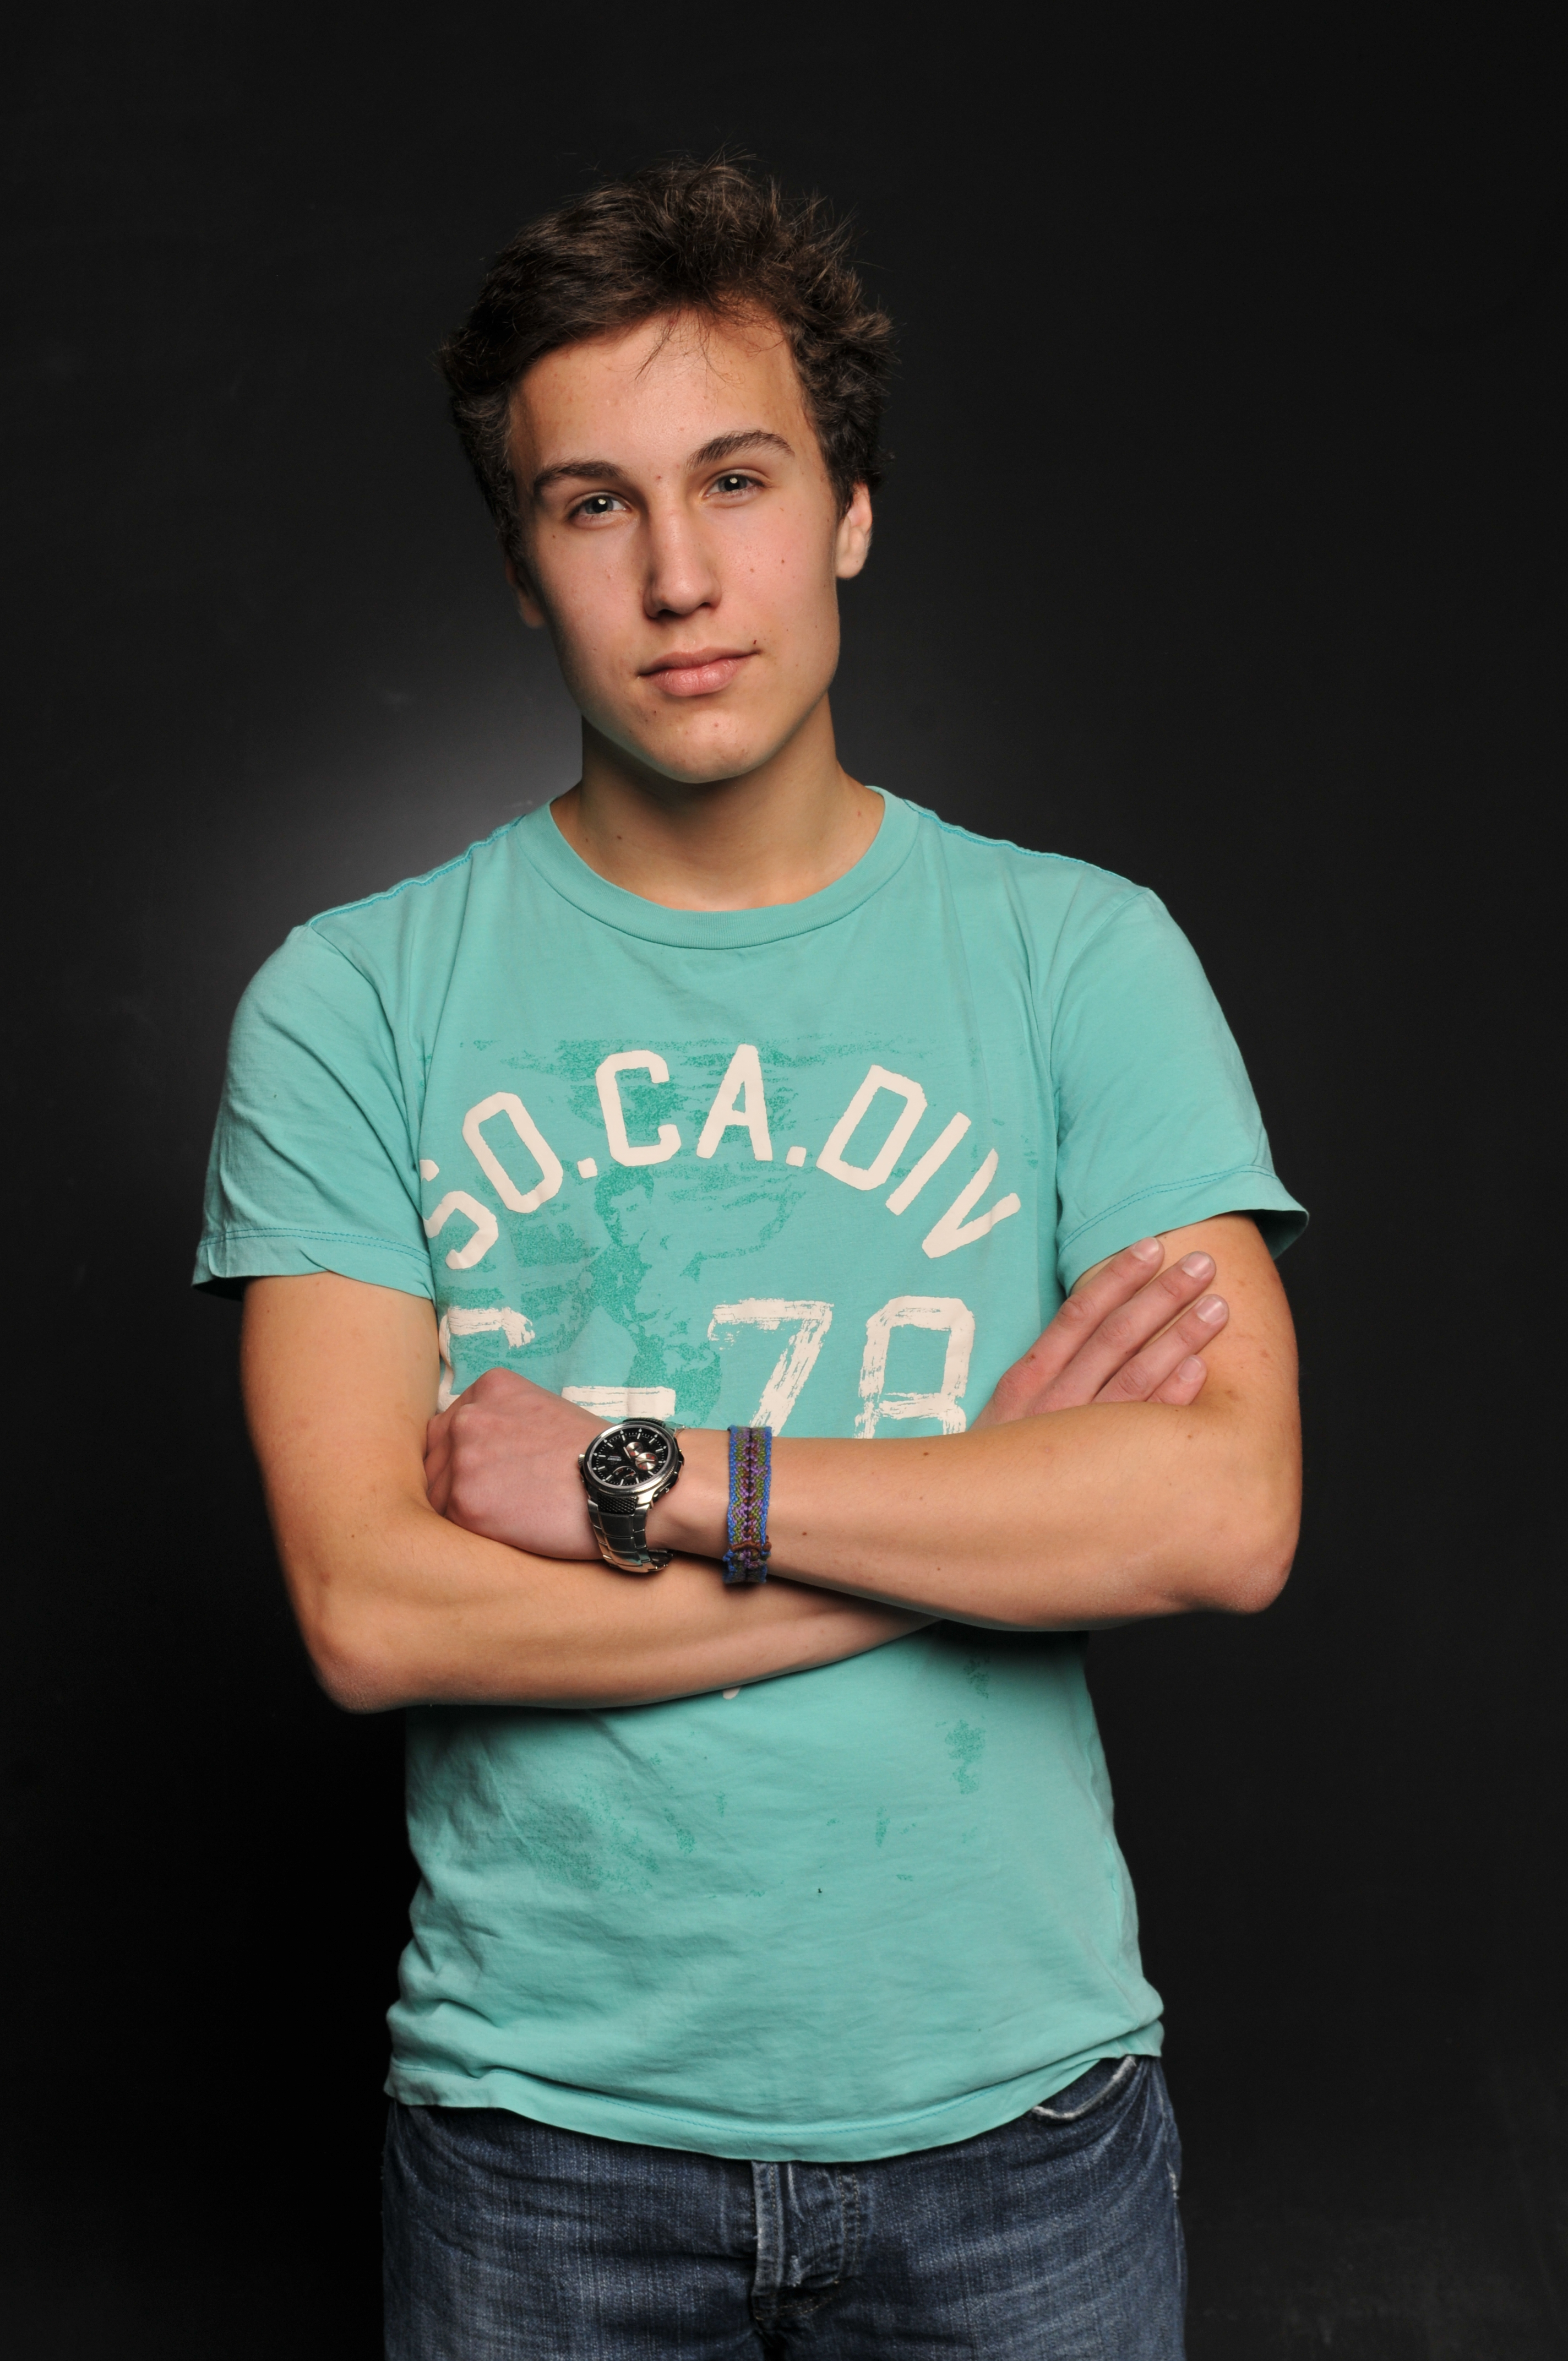
\includegraphics[scale=0.2]{3Engineering/5Team_meetings/days_of_meetings/2016.02.05/images/03}}
		\caption{Protection around the bucket was adjusted}
		\label{Protection0.0}
	\end{minipage}
\end{figure}

The second problem was that the mechanism for shifting the bucket was grasping the mount which prevented if from shifting. The cause of this grasping was detected and the protection was improved. 

Another problem was that the servo that operated the bucket’s cover worked very poor. The problem was that the contact on the signal wire was bad. We couldn’t solve this problem because of no reserve servos. However, we decided to change the servo after returning home.
